\begin{frame}{Πειραματικά αποτελέσματα: CORRIDOR (sim; 1/6)}

  \begin{figure}
    \definecolor{a}{RGB}{235, 172, 35}
\definecolor{b}{RGB}{184, 0, 88}
\definecolor{c}{RGB}{0, 140, 249}

% GNUPLOT: LaTeX picture with Postscript
\begingroup
  \makeatletter
  \providecommand\color[2][]{%
    \GenericError{(gnuplot) \space\space\space\@spaces}{%
      Package color not loaded in conjunction with
      terminal option `colourtext'%
    }{See the gnuplot documentation for explanation.%
    }{Either use 'blacktext' in gnuplot or load the package
      color.sty in LaTeX.}%
    \renewcommand\color[2][]{}%
  }%
  \providecommand\includegraphics[2][]{%
    \GenericError{(gnuplot) \space\space\space\@spaces}{%
      Package graphicx or graphics not loaded%
    }{See the gnuplot documentation for explanation.%
    }{The gnuplot epslatex terminal needs graphicx.sty or graphics.sty.}%
    \renewcommand\includegraphics[2][]{}%
  }%
  \providecommand\rotatebox[2]{#2}%
  \@ifundefined{ifGPcolor}{%
    \newif\ifGPcolor
    \GPcolorfalse
  }{}%
  \@ifundefined{ifGPblacktext}{%
    \newif\ifGPblacktext
    \GPblacktexttrue
  }{}%
  % define a \g@addto@macro without @ in the name:
  \let\gplgaddtomacro\g@addto@macro
  % define empty templates for all commands taking text:
  \gdef\gplfronttext{}%
  \gdef\gplfronttext{}%
  \makeatother
  \ifGPblacktext
    % no textcolor at all
    \def\colorrgb#1{}%
    \def\colorgray#1{}%
  \else
    % gray or color?
    \ifGPcolor
      \def\colorrgb#1{\color[rgb]{#1}}%
      \def\colorgray#1{\color[gray]{#1}}%
      \expandafter\def\csname LTw\endcsname{\color{white}}%
      \expandafter\def\csname LTb\endcsname{\color{black}}%
      \expandafter\def\csname LTa\endcsname{\color{black}}%
      \expandafter\def\csname LT0\endcsname{\color[rgb]{1,0,0}}%
      \expandafter\def\csname LT1\endcsname{\color[rgb]{0,1,0}}%
      \expandafter\def\csname LT2\endcsname{\color[rgb]{0,0,1}}%
      \expandafter\def\csname LT3\endcsname{\color[rgb]{1,0,1}}%
      \expandafter\def\csname LT4\endcsname{\color[rgb]{0,1,1}}%
      \expandafter\def\csname LT5\endcsname{\color[rgb]{1,1,0}}%
      \expandafter\def\csname LT6\endcsname{\color[rgb]{0,0,0}}%
      \expandafter\def\csname LT7\endcsname{\color[rgb]{1,0.3,0}}%
      \expandafter\def\csname LT8\endcsname{\color[rgb]{0.5,0.5,0.5}}%
    \else
      % gray
      \def\colorrgb#1{\color{black}}%
      \def\colorgray#1{\color[gray]{#1}}%
      \expandafter\def\csname LTw\endcsname{\color{white}}%
      \expandafter\def\csname LTb\endcsname{\color{black}}%
      \expandafter\def\csname LTa\endcsname{\color{black}}%
      \expandafter\def\csname LT0\endcsname{\color{black}}%
      \expandafter\def\csname LT1\endcsname{\color{black}}%
      \expandafter\def\csname LT2\endcsname{\color{black}}%
      \expandafter\def\csname LT3\endcsname{\color{black}}%
      \expandafter\def\csname LT4\endcsname{\color{black}}%
      \expandafter\def\csname LT5\endcsname{\color{black}}%
      \expandafter\def\csname LT6\endcsname{\color{black}}%
      \expandafter\def\csname LT7\endcsname{\color{black}}%
      \expandafter\def\csname LT8\endcsname{\color{black}}%
    \fi
  \fi
    \setlength{\unitlength}{0.0500bp}%
    \ifx\gptboxheight\undefined%
      \newlength{\gptboxheight}%
      \newlength{\gptboxwidth}%
      \newsavebox{\gptboxtext}%
    \fi%
    \setlength{\fboxrule}{0.5pt}%
    \setlength{\fboxsep}{1pt}%
\begin{picture}(9500.00,4000.00)%
    \gplgaddtomacro\gplfronttext{%
      \colorrgb{0.15,0.15,0.15}%
      \put(818,1902){\makebox(0,0)[r]{\strut{}4}}%
      \colorrgb{0.15,0.15,0.15}%
      \put(818,2194){\makebox(0,0)[r]{\strut{}6}}%
      \colorrgb{0.15,0.15,0.15}%
      \put(818,2486){\makebox(0,0)[r]{\strut{}8}}%
      \colorrgb{0.15,0.15,0.15}%
      \put(818,2779){\makebox(0,0)[r]{\strut{}10}}%
      \colorrgb{0.15,0.15,0.15}%
      \put(818,3071){\makebox(0,0)[r]{\strut{}12}}%
      \colorrgb{0.15,0.15,0.15}%
      \put(818,3363){\makebox(0,0)[r]{\strut{}14}}%
      \colorrgb{0.15,0.15,0.15}%
      \put(950,1536){\makebox(0,0){\strut{}2}}%
      \colorrgb{0.15,0.15,0.15}%
      \put(1242,1536){\makebox(0,0){\strut{}4}}%
      \colorrgb{0.15,0.15,0.15}%
      \put(1534,1536){\makebox(0,0){\strut{}6}}%
      \colorrgb{0.15,0.15,0.15}%
      \put(1826,1536){\makebox(0,0){\strut{}8}}%
      \colorrgb{0.15,0.15,0.15}%
      \put(2119,1536){\makebox(0,0){\strut{}10}}%
      \colorrgb{0.15,0.15,0.15}%
      \put(2411,1536){\makebox(0,0){\strut{}12}}%
      \colorrgb{0.15,0.15,0.15}%
      \put(2703,1536){\makebox(0,0){\strut{}14}}%
    }%
    \gplgaddtomacro\gplfronttext{%
      \colorrgb{0.15,0.15,0.15}%
      \put(312,2632){\rotatebox{90}{\makebox(0,0){\strut{}$y$ [m]}}}%
      \colorrgb{0.15,0.15,0.15}%
      \put(1899,1206){\makebox(0,0){\strut{}$x$ [m]}}%
      \put(1899,300){\makebox(0,0){\strut{}$|\mathcal{H}_C| = 100$ υποθέσεις}}%
    }%
    \gplgaddtomacro\gplfronttext{%
      \colorrgb{0.15,0.15,0.15}%
      \put(3668,2933){\makebox(0,0)[r]{\strut{}\scriptsize $0\%$}}%
      \colorrgb{0.15,0.15,0.15}%
      \put(3668,3100){\makebox(0,0)[r]{\strut{}\scriptsize $25\%$}}%
      \colorrgb{0.15,0.15,0.15}%
      \put(3668,3266){\makebox(0,0)[r]{\strut{}\scriptsize $50\%$}}%
      \colorrgb{0.15,0.15,0.15}%
      \put(3668,3433){\makebox(0,0)[r]{\strut{}\scriptsize $75\%$}}%
      \colorrgb{0.15,0.15,0.15}%
      \put(3668,3599){\makebox(0,0)[r]{\strut{}\scriptsize $100\%$}}%
      \colorrgb{0.15,0.15,0.15}%
      \put(4117,2813){\makebox(0,0){\strut{}\scriptsize \textcolor{a}{$\bm{p}_a^C$}}}%
      \colorrgb{0.15,0.15,0.15}%
      \put(4750,2813){\makebox(0,0){\strut{}\scriptsize \textcolor{b}{$\bm{p}_b^C$}}}%
      \colorrgb{0.15,0.15,0.15}%
      \put(5383,2813){\makebox(0,0){\strut{}\scriptsize \textcolor{c}{$\bm{p}_c^C$}}}%
    }%
    \gplgaddtomacro\gplfronttext{%
      \colorrgb{0.00,0.00,0.00}%
      \put(6000,3819){\makebox(0,0){\strut{}\footnotesize Ποσοστά αποτυχιών}}%
    }%
    \gplgaddtomacro\gplfronttext{%
      \colorrgb{0.15,0.15,0.15}%
      \put(6518,2933){\makebox(0,0)[r]{\strut{}\scriptsize $0\%$}}%
      \colorrgb{0.15,0.15,0.15}%
      \put(6518,3100){\makebox(0,0)[r]{\strut{}\scriptsize $25\%$}}%
      \colorrgb{0.15,0.15,0.15}%
      \put(6518,3266){\makebox(0,0)[r]{\strut{}\scriptsize $50\%$}}%
      \colorrgb{0.15,0.15,0.15}%
      \put(6518,3433){\makebox(0,0)[r]{\strut{}\scriptsize $75\%$}}%
      \colorrgb{0.15,0.15,0.15}%
      \put(6518,3599){\makebox(0,0)[r]{\strut{}\scriptsize $100\%$}}%
      \colorrgb{0.15,0.15,0.15}%
      \put(6967,2813){\makebox(0,0){\strut{}\scriptsize \textcolor{a}{$\bm{p}_a^C$}}}%
      \colorrgb{0.15,0.15,0.15}%
      \put(7600,2813){\makebox(0,0){\strut{}\scriptsize \textcolor{b}{$\bm{p}_b^C$}}}%
      \colorrgb{0.15,0.15,0.15}%
      \put(8233,2813){\makebox(0,0){\strut{}\scriptsize \textcolor{c}{$\bm{p}_c^C$}}}%
    }%
    \gplgaddtomacro\gplfronttext{%
    }%
    \gplgaddtomacro\gplfronttext{%
      \colorrgb{0.15,0.15,0.15}%
      \put(3668,1666){\makebox(0,0)[r]{\strut{}\scriptsize $0.0$}}%
      \colorrgb{0.15,0.15,0.15}%
      \put(3668,1799){\makebox(0,0)[r]{\strut{}\scriptsize $0.01$}}%
      \colorrgb{0.15,0.15,0.15}%
      \put(3668,1932){\makebox(0,0)[r]{\strut{}\scriptsize $0.02$}}%
      \colorrgb{0.15,0.15,0.15}%
      \put(3668,2066){\makebox(0,0)[r]{\strut{}\scriptsize $0.03$}}%
      \colorrgb{0.15,0.15,0.15}%
      \put(3668,2199){\makebox(0,0)[r]{\strut{}\scriptsize $0.04$}}%
      \colorrgb{0.15,0.15,0.15}%
      \put(3668,2332){\makebox(0,0)[r]{\strut{}\scriptsize $0.05$}}%
      \colorrgb{0.15,0.15,0.15}%
      \put(3717,1546){\makebox(0,0){\strut{}\scriptsize $\sigma_R$:}}%
      \put(4117,1546){\makebox(0,0){\strut{}\scriptsize $0.01$}}%
      \colorrgb{0.15,0.15,0.15}%
      \put(4750,1546){\makebox(0,0){\strut{}\scriptsize $0.02$}}%
      \colorrgb{0.15,0.15,0.15}%
      \put(5383,1546){\makebox(0,0){\strut{}\scriptsize $0.05$}}%
    }%
    \gplgaddtomacro\gplfronttext{%
      \colorrgb{0.00,0.00,0.00}%
      \put(6000,2552){\makebox(0,0){\strut{}\footnotesize Μέσο σφάλμα στάσης [$(\text{m}^2 + \text{rad}^2)^{1/2}$]}}%
    }%
    \gplgaddtomacro\gplfronttext{%
      \colorrgb{0.15,0.15,0.15}%
      \put(6518,1666){\makebox(0,0)[r]{\strut{}\scriptsize $0.0$}}%
      \colorrgb{0.15,0.15,0.15}%
      \put(6518,1799){\makebox(0,0)[r]{\strut{}\scriptsize $0.01$}}%
      \colorrgb{0.15,0.15,0.15}%
      \put(6518,1932){\makebox(0,0)[r]{\strut{}\scriptsize $0.02$}}%
      \colorrgb{0.15,0.15,0.15}%
      \put(6518,2066){\makebox(0,0)[r]{\strut{}\scriptsize $0.03$}}%
      \colorrgb{0.15,0.15,0.15}%
      \put(6518,2199){\makebox(0,0)[r]{\strut{}\scriptsize $0.04$}}%
      \colorrgb{0.15,0.15,0.15}%
      \put(6518,2332){\makebox(0,0)[r]{\strut{}\scriptsize $0.05$}}%
      \colorrgb{0.15,0.15,0.15}%
      \put(6567,1546){\makebox(0,0){\strut{}\scriptsize $\sigma_R$:}}%
      \put(6967,1546){\makebox(0,0){\strut{}\scriptsize $0.01$}}%
      \colorrgb{0.15,0.15,0.15}%
      \put(7600,1546){\makebox(0,0){\strut{}\scriptsize $0.02$}}%
      \colorrgb{0.15,0.15,0.15}%
      \put(8233,1546){\makebox(0,0){\strut{}\scriptsize $0.05$}}%
    }%
    \gplgaddtomacro\gplfronttext{%
    }%
    \gplgaddtomacro\gplfronttext{%
      \colorrgb{0.15,0.15,0.15}%
      \put(3668,400){\makebox(0,0)[r]{\strut{}\scriptsize $160$}}%
      \colorrgb{0.15,0.15,0.15}%
      \put(3668,567){\makebox(0,0)[r]{\strut{}\scriptsize $200$}}%
      \colorrgb{0.15,0.15,0.15}%
      \put(3668,733){\makebox(0,0)[r]{\strut{}\scriptsize $240$}}%
      \colorrgb{0.15,0.15,0.15}%
      \put(3668,900){\makebox(0,0)[r]{\strut{}\scriptsize $280$}}%
      \colorrgb{0.15,0.15,0.15}%
      \put(3668,1066){\makebox(0,0)[r]{\strut{}\scriptsize $320$}}%
      \colorrgb{0.15,0.15,0.15}%
      \put(3717,280){\makebox(0,0){\strut{}\scriptsize $\sigma_R$:}}%
      \put(4117,280){\makebox(0,0){\strut{}\scriptsize $0.01$}}%
      \colorrgb{1.15,0.15,0.15}%
      \put(4750,280){\makebox(0,0){\strut{}\scriptsize $0.02$}}%
      \colorrgb{1.15,0.15,0.15}%
      \put(5383,280){\makebox(0,0){\strut{}\scriptsize $0.05$}}%
    }%
    \gplgaddtomacro\gplfronttext{%
      \colorrgb{0.00,0.00,0.00}%
      \put(6000,1286){\makebox(0,0){\strut{}\footnotesize Μέσος χρόνος εκτέλεσης ανά υπόθεση [ms]}}%
    }%
    \gplgaddtomacro\gplfronttext{%
      \colorrgb{0.15,0.15,0.15}%
      \put(6518,400){\makebox(0,0)[r]{\strut{}\scriptsize $160$}}%
      \colorrgb{0.15,0.15,0.15}%
      \put(6518,567){\makebox(0,0)[r]{\strut{}\scriptsize $200$}}%
      \colorrgb{0.15,0.15,0.15}%
      \put(6518,733){\makebox(0,0)[r]{\strut{}\scriptsize $240$}}%
      \colorrgb{0.15,0.15,0.15}%
      \put(6518,900){\makebox(0,0)[r]{\strut{}\scriptsize $208$}}%
      \colorrgb{0.15,0.15,0.15}%
      \put(6518,1066){\makebox(0,0)[r]{\strut{}\scriptsize $320$}}%
      \colorrgb{0.15,0.15,0.15}%
      \put(6567,280){\makebox(0,0){\strut{}\scriptsize $\sigma_R$:}}%
      \put(6967,280){\makebox(0,0){\strut{}\scriptsize $0.01$}}%
      \colorrgb{1.15,0.15,0.15}%
      \put(7600,280){\makebox(0,0){\strut{}\scriptsize $0.02$}}%
      \colorrgb{1.15,0.15,0.15}%
      \put(8233,280){\makebox(0,0){\strut{}\scriptsize $0.05$}}%
    }%
    \gplgaddtomacro\gplfronttext{%
    }%
    \put(0,0){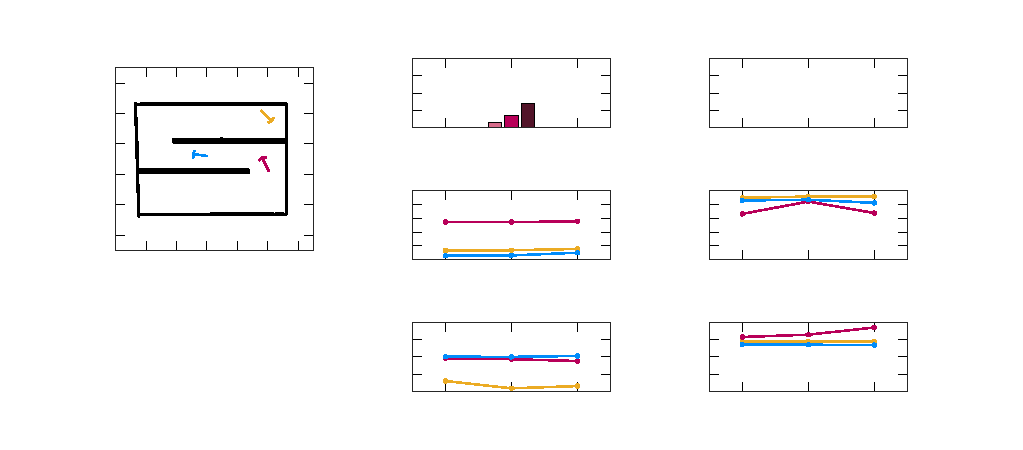
\includegraphics{./figures/slides/ch5/experiments//results_corridor}}%
    \gplfronttext
  \end{picture}%
\endgroup

  \end{figure}


\note{\footnotesize
Σε όλα τα πειράματα δοκιμάζουμε δύο υποκείμενες μεθόδους sm2. Από τη μία
  δοκιμάζουμε την καλύτερη μέθοδο της βιβλιογραφίας, δηλάδη την plicp που
  είδαμε και πριν, και από την αλλη τη μέθοδο που αποτελείται από τον FMI-SPOMF
  σε συνδυασμό με τη μέθοδο των κεντροειδών. Σε αυτή τη διαφάνεια βλέπουμε τα
  αποτελέσματα στο προσομοιωμένο περιβάλλον corridor. Στην πάνω σειρά βλέπουμε
  τα ποσοστά αποτυχημένων εκτιμήσεων στάσης, στη δεύτερη σειρά το μέσο σφάλμα
  στάσης ανά τιμή τυπικής απόκλισης μετρητικού θορύβου, και στην κάτω σειρά
  απεικονίζονται οι χρόνοι εκτέλεσης των μεθόδων ανά υπόθεση. Αυτή η διαφάνεια
  συνοψίζει αυτά που θα δούμε και στις επόμενες, δηλαδή πως ο plicp εμφανίζει
  μεγαλύτερα ποσοστά αποτυχιών ανέυρεσης της στάσης του αισθητήρα, πως τα
  σφάλματα του FMI-SPOMF είναι της ίδιας τάξης μεγέθους με αυτά του plicp, και
  πως ο χρόνος εκτέλεσής του είναι της ίδιας τάξης αλλά ελαφρώς μεγαλύτερος από
  αυτόν του plicp.}
\end{frame}
